% Created 2020-07-23 jue 12:06
% Intended LaTeX compiler: pdflatex
\documentclass[presentation,aspectratio=169]{beamer}
\usepackage[utf8]{inputenc}
\usepackage[T1]{fontenc}
\usepackage{graphicx}
\usepackage{grffile}
\usepackage{longtable}
\usepackage{wrapfig}
\usepackage{rotating}
\usepackage[normalem]{ulem}
\usepackage{amsmath}
\usepackage{textcomp}
\usepackage{amssymb}
\usepackage{capt-of}
\usepackage{hyperref}
\usepackage{khpreamble}
\usepackage{amssymb}
\usepackage{pgfplotstable}
\DeclareMathOperator{\shift}{q}
\DeclareMathOperator{\diff}{p}
\usetheme{default}
\author{Kjartan Halvorsen}
\date{\today}
\title{Control computarizado - Identificación de sistemas}
\hypersetup{
 pdfauthor={Kjartan Halvorsen},
 pdftitle={Control computarizado - Identificación de sistemas},
 pdfkeywords={},
 pdfsubject={},
 pdfcreator={Emacs 26.3 (Org mode 9.3.6)}, 
 pdflang={English}}
\begin{document}

\maketitle

\section{Retroalimentacion Tarea 3}
\label{sec:org14bb150}

\begin{frame}[label={sec:org1b780b1}]{Retroalimentación Tarea 3}
\end{frame}

\begin{frame}[label={sec:org3dbf91d}]{Retroalimentación Tarea 3}
\begin{itemize}
\item Dominan el diseño del controlador RST
\item Retos en la implementacion y simulacion en simulink
\end{itemize}
\end{frame}

\section{Intro}
\label{sec:org08be703}
\begin{frame}[label={sec:orgdddf6e3}]{Identificación de sistemas}
\end{frame}
\begin{frame}[label={sec:org7073d5c}]{Identificación de sistemas}
\begin{center}
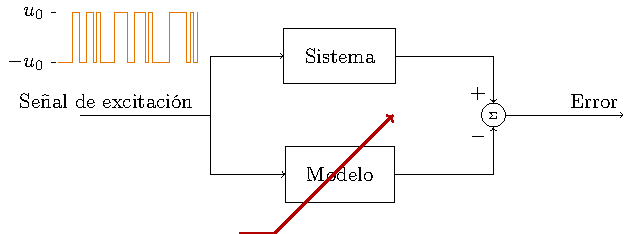
\includegraphics[]{sysid-graphic} 
\end{center}
\end{frame}

\section{ARX-model}
\label{sec:orga698171}

\begin{frame}[label={sec:org90965b8}]{Model AutoRegresivo con variables eXógenas (ARX)}
Dado señal discreta de entrada de un sistema \(u(k), \; k=1,2,\ldots, N\) y observaciones de la respuesta \(y(k), \; k=1,2,\ldots,N\), y el modelo ARX
\[ A(\shift) y(k) = B(\shift)u(k) + e(k+n),\]
dónde \(e(k)\) es una sequencia discreta de ruido blanco.
\begin{center}
  \begin{tikzpicture}[node distance=22mm, block/.style={rectangle, draw, minimum width=15mm, minimum height=12mm}, sumnode/.style={circle, draw, inner sep=2pt}]
    
    \node[coordinate] (input) {};
    \node[block, right of=input, node distance=20mm] (plant)  {$\frac{B(z)}{A(z)}$};
    \node[sumnode, right of=plant, node distance=24mm] (sum) {\tiny $\Sigma$};
    \node[block, above of=sum, node distance=20mm] (dist)  {$\frac{z^n}{A(z)}$};

    \node[coordinate, above of=dist, node distance=12mm] (disturbance) {};
    \node[coordinate, right of=sum, node distance=20mm] (output) {};

    \draw[->] (input) -- node[above, pos=0.3] {$u(k)$} (plant);
    \draw[->] (plant) -- node[above] {} (sum);
    \draw[->] (sum) -- node[above, near end] {$y(k)$} (output);
    \draw[->] (disturbance) -- node[right, pos=0.2] {$e(k)$} (dist);
    \draw[->] (dist) -- node[above] {} (sum);

  \end{tikzpicture}
\end{center}
\end{frame}
\begin{frame}[label={sec:org9eca465}]{Model ARX de orden \(n\)}
Dado señal discreta de entrada de un sistema \(u(k), \; k=1,2,\ldots, N\) y observaciones de la respuesta \(y(k), \; k=1,2,\ldots,N\), el modelo ARX \(A(\shift)y(k) = B(\shift)u(k-d) + \shift^n e(k)\) con \(n\) polos, \(m\) ceros y retraso de \(d\) pasos

\alert{Predictor}
\begin{multline*}
\hat{y}(k+1) = -a_1y(k) - \cdots - a_ny(k-n+1) \\+ b_0u(k+m-n-d+1) + \cdots + b_mu(k-n-d+1)  +   e(k+1)
\end{multline*}


\alert{Objetivo} Estimar los parametro \(a_1, a_2, \ldots, \a_n, b_0, b_1, \ldots, b_m\).
\end{frame}

\begin{frame}[label={sec:org47900cd}]{Ejemplo y tarea}
\href{https://mybinder.org/v2/gh/kjartan-at-tec/mr2007-computerized-control/master?filepath=system-identification\%2Fnotebooks\%2FParameter\%20estimation\%20with\%20least\%20squares.ipynb}{Ejercicios}

\href{https://mybinder.org/v2/gh/kjartan-at-tec/mr2007-computerized-control/master?filepath=system-identification\%2Fnotebooks\%2FParameter\%20estimation\%20with\%20least\%20squares\%20-\%20Homework.ipynb}{Tarea}
\end{frame}
\end{document}